\documentclass[10pt]{article}
\usepackage[margin=1in]{geometry}
\usepackage{amsmath}
\usepackage{amssymb}
\usepackage[T1]{fontenc}
\usepackage{lmodern}
\usepackage{microtype}
\usepackage{array}
\usepackage{algorithm}
\usepackage{algpseudocode}
\usepackage{tikz}
\usetikzlibrary{arrows.meta,positioning,shapes.geometric,calc}

\setlength{\parindent}{0pt}
\setlength{\parskip}{0.7\baselineskip}

\title{A Practical Method for Detecting Secrets in Environment Variables (Application Note, 2026 v1.0)}
\author{Jonas \r{A}str\"om}
\date{}

\begin{document}

\maketitle

\textbf{Abstract.} This application note presents an implementation-oriented method for estimating secret probability in environment variables (e.g., API keys, access tokens, and strong passwords) in real screening pipelines. The method combines permutation-aware entropy diagnostics with Bayesian evidence fusion; to our knowledge, this specific combination (permutation-aware entropy baselines plus Bayesian posterior evidence updates for environment-variable screening) is not standard in widely used secret-scanning tools. The presentation includes a practical hypothesis-testing interpretation in which a permutation-derived statistic serves as the test quantity and is approximated in practice with a fixed small number of permutations, yielding an interpretable and reproducible detector.

\section*{Problem Setting}

Given an environment entry of the form \texttt{NAME=VALUE}, the goal is to estimate
\[
P(\text{secret}\mid\text{evidence from NAME and VALUE}).
\]
The method is designed to reduce both false positives (paths, standard shell variables) and false negatives (high-entropy but structured credentials).

Throughout, $S$ denotes a candidate value string; $H_1$ and $H_2$ denote character-level and 2-gram entropy; $R_c$ and $R_2$ denote entropy ratios against permutation baselines; and $P(\text{secret})$ denotes the posterior after sequential evidence updates.

\section*{Positioning with Prior Work}

This application note reports a practical implementation. Prior empirical work has documented the prevalence and impact of secret leakage in public repositories~[3], and follow-up studies have shown that deployment challenges extend beyond raw false-positive rates~[4]. In operational tooling, our method sits alongside established scanners such as GitHub Secret Scanning~[5], Yelp's \texttt{detect-secrets}~[6], and \texttt{gitleaks}~[7]. Public documentation and maintainer descriptions indicate that common approaches rely on regex/rule matching, entropy thresholds, and allowlists (for example, in \texttt{gitleaks})~[8], while permutation-based entropy baselines are not explicitly described. The focus here is an explicit, reproducible combination of permutation-aware entropy features and Bayesian evidence fusion for environment-variable screening.

Table~\ref{tab:method-comparison} gives a scope-focused comparison: many established tools target broad repository/text scanning and operational integration, whereas this note isolates scoring for \texttt{NAME=VALUE} screening and emphasizes a fused, permutation-calibrated evidence model over plain Shannon-only scoring.

\begin{table}[ht]
\centering
\begin{tabular}{|>{\raggedright\arraybackslash}p{3.1cm}|>{\raggedright\arraybackslash}p{3.1cm}|>{\raggedright\arraybackslash}p{5.2cm}|>{\raggedright\arraybackslash}p{3.1cm}|}
\hline
\textbf{Approach class} & \textbf{Primary scope} & \textbf{Indicators / statistics} & \textbf{Inference model} \\
\hline
Repository secret scanners (e.g., GitHub Secret Scanning~[5], \texttt{detect-secrets}~[6], \texttt{gitleaks}~[7,8]) & Large-text/repository detection plus operational workflow concerns & Rule/pattern matching, entropy-threshold heuristics, and allowlist controls for practical detection pipelines & Rule- and heuristic-driven scoring designed for actionable detection decisions in operational workflows \\
\hline
This application note (environment-variable scorer) & Focused \texttt{NAME=VALUE} scoring method, separated from broader systems pipeline concerns & Deterministic permutation-normalized conditional-entropy and 2-gram entropy ratios ($R_c$, $R_2$), alongside Shannon entropy ($H_1$) & Interpretable Bayesian posterior updates over entropy and non-entropy cues \\
\hline
\end{tabular}
\caption{Scope and method comparison between broad secret-scanning tool classes and the scoring method documented here.}
\label{tab:method-comparison}
\end{table}

\section*{Entropy Features and Test Statistics}

The detector computes four entropy-based features from the value string:

\textbf{1) Shannon entropy} $H_1$ on characters.
For a character distribution $p(x)$ over the string,
\[
H_1 = -\sum_x p(x)\log_2 p(x).
\]

\textbf{2) 2-gram entropy} $H_2$.
Let $p_2(x,y)$ denote the empirical distribution of adjacent character pairs; then
\[
H_2 = -\sum_{x,y} p_2(x,y)\log_2 p_2(x,y).
\]

\textbf{3) Relative conditional entropy ratio}
\[
R_c = \frac{H(X_i\mid X_{i-1})}{\operatorname{median}_{\pi} H\!\left(X_i^{\pi}\mid X_{i-1}^{\pi}\right)}.
\]
Here,
\[
H(X_i\mid X_{i-1}) = -\sum_{x,y} p(x,y)\log_2 p(y\mid x),
\]
with $p(x,y)$ estimated from adjacent character pairs in the string.
Here, $\pi$ denotes a deterministic pseudo-random permutation of character order. If the denominator collapses to zero, the implementation returns a sentinel ratio of $2.0$.

\textbf{4) Relative 2-gram entropy ratio}
\[
R_2 = \frac{H_2(\text{original})}{\operatorname{median}_{\pi} H_2(\text{permuted})},
\]
with the same deterministic permutation scheme.

Thus, permutation calibration is applied to both sequence-sensitive features: conditional 1-gram entropy (via $R_c$) and adjacent 2-gram entropy (via $R_2$). The current fusion layer then treats these as separate evidence terms and updates the posterior sequentially (one Bayes update per feature), together with normalized $H_1$ and later name/format cues.

For short strings (length $<12$), the method falls back to direct entropy (without permutation), avoiding unstable statistics.

These ratios can be interpreted as test statistics for deviation from a permutation-based null reference.

\section*{Hypothesis-Testing Formalization (Practical Form)}

Let $S$ be a value string, and let $T(S)$ be a statistic such as $R_c$ or $R_2$.
Define hypotheses
\[
H_0:\ \text{non-secret-like generation} \quad\text{vs.}\quad H_1:\ \text{secret-like generation}.
\]

Using a permutation reference distribution $\{T(S^{\pi_b})\}_{b=1}^B$, a two-sided permutation-style p-value can be written as
\[
\hat p_B = \frac{1 + \sum_{b=1}^{B}\mathbf{1}\!\left\{\left|T(S^{\pi_b})-\mu_B\right| \geq \left|T(S)-\mu_B\right|\right\}}{B+1},
\]
where $\mu_B$ is the empirical center (e.g., median) of the permuted statistics.

In the current implementation, this idealized test is approximated with a fixed, small $B$ (typically 5 or 10) and summarized through robust ratios (median-normalized entropy statistics) rather than explicit p-values. In practice, permutation testing is used mainly as a calibration mechanism for stable feature construction, and $R_c$ and $R_2$ can be treated as calibrated summary features without computing explicit p-values.

\section*{Deterministic Permutation Procedure}

For each permutation index, a seeded Fisher--Yates shuffle generates a reproducible rearrangement of the string. The implementation evaluates entropy across several such permutations (typically 5 or 10) and uses the median as a robust baseline.

Empirically, secrets often preserve near-random behavior even after permutation, whereas structured non-secrets can exhibit larger deviations from the permuted baseline.

For finite $B$, Monte Carlo approximation error decreases as $B$ grows. In this specific setting, each summand
\[
I_b = \mathbf{1}\!\left\{\left|T(S^{\pi_b})-\mu_B\right| \geq \left|T(S)-\mu_B\right|\right\}
\]
is an indicator variable, so $I_b\in\{0,1\}$ and is therefore bounded. If permutations are sampled independently (or are sufficiently decorrelated in practice), then $\{I_b\}$ behaves as Bernoulli draws with mean equal to the tail probability being estimated. Hence, standard concentration bounds (e.g., Hoeffding's inequality) apply~[1,2]:
\[
\Pr\!\left(\left|\frac{1}{B}\sum_{b=1}^B I_b - \mathbb{E}[I_b]\right|\ge \varepsilon\right)
\le 2\exp(-2B\varepsilon^2).
\]
This yields a typical estimation error of order $O(B^{-1/2})$, clarifying the speed--accuracy tradeoff when choosing small fixed $B$.

\section*{Assumptions and Limitations}

The method relies on several practical assumptions that should be made explicit:
\begin{itemize}
  \item \textbf{Permutation sampling assumption:} the concentration statement for $\hat p_B$ is exact under independent permutation samples; deterministic seeded permutations are used here as a practical approximation.
  \item \textbf{Feature-likelihood calibration:} Bayesian likelihood functions are currently heuristic and should be re-calibrated when deployment domains change.
  \item \textbf{Short-string regime:} when length $<12$, permutation features are bypassed; decisions then rely more heavily on Shannon entropy and non-entropy cues.
  \item \textbf{Domain drift risk:} naming conventions, token formats, and path conventions can evolve over time, requiring periodic updates to prefixes, patterns, and thresholds.
\end{itemize}

\section*{Bayesian Evidence Fusion Layer}

The model uses a prior
\[
P(\text{secret}) = 0.10
\]
and updates it sequentially with likelihood models.

\textbf{Entropy likelihoods:}
\begin{itemize}
  \item The model computes three entropy-derived evidence terms: normalized Shannon entropy $H_1$, permutation-calibrated conditional 1-gram ratio $R_c$, and permutation-calibrated 2-gram ratio $R_2$.
  \item Ratios near $1.0$ are modeled as more likely under the secret hypothesis using a Gaussian-like likelihood.
  \item Ratios far from $1.0$ increase non-secret likelihood via a bimodal distance-based function.
  \item Normalized Shannon entropy is mapped through sigmoids for secret and non-secret likelihoods.
  \item In the default implementation, these entropy terms are fused with equal structural weight by applying one sequential Bayes update per term (rather than an extra manual weighting coefficient).
\end{itemize}

\textbf{Likelihood design rationale.}
The selected functional forms encode practical inductive bias while keeping the model interpretable:
\begin{itemize}
  \item \textbf{Ratio terms centered at 1.0:} if a value remains statistically similar under permutation, the ratio tends to stay near 1.0; this motivates a secret-likelihood peak around 1.0.
  \item \textbf{Distance-based non-secret model:} larger deviations $|r-1|$ are treated as stronger evidence of structure, motivating a non-secret likelihood that increases away from the center.
  \item \textbf{Sigmoid for normalized Shannon entropy:} smooth monotone mapping avoids hard cutoffs and reflects that higher normalized entropy generally supports the secret hypothesis.
  \item \textbf{Floors and ceilings on likelihoods:} bounded likelihood values prevent single features from numerically dominating all subsequent updates.
\end{itemize}
These parameter values are heuristic, implementation-oriented defaults; in deployment they should be re-estimated or calibrated on labeled data.

\textbf{Independence and ordering caveat.}
Sequential Bayes updates are exact only when likelihood terms are conditionally independent given the hypothesis. In practice, entropy, name-pattern, and prefix features are partially correlated, so unless a joint model or dependency correction is introduced, the resulting posterior is best interpreted as a calibrated score rather than a strictly coherent posterior probability.

\textbf{Name and format evidence mapped to likelihoods.}
Additional non-entropy evidence is incorporated as explicit likelihood terms:
\begin{itemize}
  \item Known secret prefixes in values (e.g., \texttt{sk\_}, \texttt{AKIA}, \texttt{ghp\_}) map to high secret likelihood and low non-secret likelihood.
  \item Secret-like variable names (containing terms such as \texttt{KEY}, \texttt{TOKEN}, \texttt{PASSWORD}) map to higher secret likelihood.
  \item Path-like values (e.g., \texttt{/home/...}, \texttt{/tmp/...}) map to high non-secret likelihood and low secret likelihood.
\end{itemize}

Each evidence source is incorporated via Bayes updates:
\[
P' = \frac{P\,L_s}{P\,L_s + (1-P)\,L_{\neg s}},
\]
where $L_s$ and $L_{\neg s}$ are likelihoods under secret and non-secret hypotheses.

\section*{Screening Pipeline}

For each environment variable:
\begin{enumerate}
  \item Split into \texttt{name} and \texttt{value}.
  \item Skip empty values, very short values, and a whitelist of common non-secret variables.
  \item Compute entropy-based posterior from $H_1$, $R_c$, and $R_2$.
  \item Update with prefix, name-pattern, and path evidence.
  \item Flag as potential secret if posterior exceeds a configurable threshold.
\end{enumerate}

For a compact operational view, Figure~\ref{fig:screening-flow} summarizes the full screening flow (including branch-specific checks and evidence fusion), Table~\ref{tab:defaults} lists practical defaults used in the current implementation, and Algorithm~\ref{alg:screening} gives step-by-step pseudocode.

\section*{Concrete Walkthroughs (Two Redacted Examples)}

This section instantiates the full pipeline on two redacted entries: one clear case and one flagged case.

\textbf{Walkthrough A (clear case): input and thresholds.}
\begin{itemize}
  \item \texttt{name = MEMORY\_PRESSURE\_WRITE}
  \item \texttt{value = [VALUE REDACTED]} (length $=28$)
  \item Minimum length threshold $=24$
  \item Decision threshold $\tau=0.50$
\end{itemize}

\textbf{Step 1: parse and prechecks.}
The variable is parsed as non-empty, not whitelisted, and above the minimum length, so scoring proceeds.

\textbf{Step 2: entropy and structure indicators.}
For the redacted value, the feature extractor reports:
\[
H_1=3.3513\ \text{bits/char},\quad \frac{H_1}{8}=0.4189,\quad R_c=0.6958,\quad R_2=0.8992.
\]
Both ratio features are below $1.0$, indicating sequence structure relative to permutation baselines. The format checks also report: no known secret prefix, no secret-like variable-name pattern, no path-like value, and base64-like format detected.

\textbf{Step 3: Bayesian evidence updates.}
Starting from prior
\[
P_0=P(\text{secret})=0.10,
\]
the entropy evidence uses the following likelihood pairs from the run output:
\begin{itemize}
  \item $R_c=0.6958$: \ $P(E\mid\text{secret})=0.2087$, \ $P(E\mid\neg\text{secret})=0.9499$
  \item $R_2=0.8992$: \ $P(E\mid\text{secret})=0.7781$, \ $P(E\mid\neg\text{secret})=0.1000$
  \item $H_1/8=0.4189$: \ $P(E\mid\text{secret})=0.1405$, \ $P(E\mid\neg\text{secret})=0.8595$
\end{itemize}
After sequential entropy and non-entropy updates (prefix absent, name-pattern absent, path absent), the final posterior reported by the run is:
\[
P_{\mathrm{final}}=0.0140.
\]

\textbf{Step 4: threshold decision.}
With threshold $\tau=0.50$,
\[
P_{\mathrm{final}}=0.0140<0.50,
\]
so the entry is classified as \emph{Do not flag} (CLEAR).

This example shows how moderate entropy, sub-unit permutation ratios, and absent secret-specific contextual signals can combine into a low posterior under the current likelihood model and thresholds.

\textbf{Walkthrough B (flagged case): input and thresholds.}
\begin{itemize}
  \item \texttt{name = MINIMAX\_API\_KEY}
  \item \texttt{value = [VALUE REDACTED]} (length $=125$)
  \item Minimum length threshold $=24$
  \item Decision threshold $\tau=0.50$
\end{itemize}

\textbf{Step 1: parse and prechecks.}
The variable is parsed as non-empty, not whitelisted, and above the minimum length, so scoring proceeds.

\textbf{Step 2: entropy and structure indicators.}
For the redacted value, the feature extractor reports suffix-based Shannon entropy (after detected prefix):
\[
H_1=5.5116\ \text{bits/char},\quad \frac{H_1}{8}=0.6890,\quad R_c=1.0209,\quad R_2=1.0047.
\]
Both ratio features are slightly above $1.0$, indicating near-random behavior relative to permutation baselines. The format checks report: known secret prefix present, secret-like variable-name pattern present, no path-like value, and not base64-like.

\textbf{Step 3: Bayesian evidence updates.}
Starting from prior
\[
P_0=P(\text{secret})=0.10,
\]
the entropy evidence uses the following likelihood pairs from the run output:
\begin{itemize}
  \item $R_c=1.0209$: \ $P(E\mid\text{secret})=0.9418$, \ $P(E\mid\neg\text{secret})=0.1000$
  \item $R_2=1.0047$: \ $P(E\mid\text{secret})=0.9496$, \ $P(E\mid\neg\text{secret})=0.1000$
  \item $H_1/8=0.6890$: \ $P(E\mid\text{secret})=0.7088$, \ $P(E\mid\neg\text{secret})=0.2912$
\end{itemize}
After sequential entropy and non-entropy updates (prefix present, name-pattern present, path absent), the final posterior reported by the run is:
\[
P_{\mathrm{final}}=1.0000.
\]

\textbf{Step 4: threshold decision.}
With threshold $\tau=0.50$,
\[
P_{\mathrm{final}}=1.0000>0.50,
\]
so the entry is classified as \emph{Flag as potential secret} (FLAGGED).

Together, these two walkthroughs illustrate both ends of the operating range under identical screening thresholds: a low-score clear case and a high-confidence flagged case.

\begin{figure}[ht]
\centering
\resizebox{0.96\linewidth}{!}{%
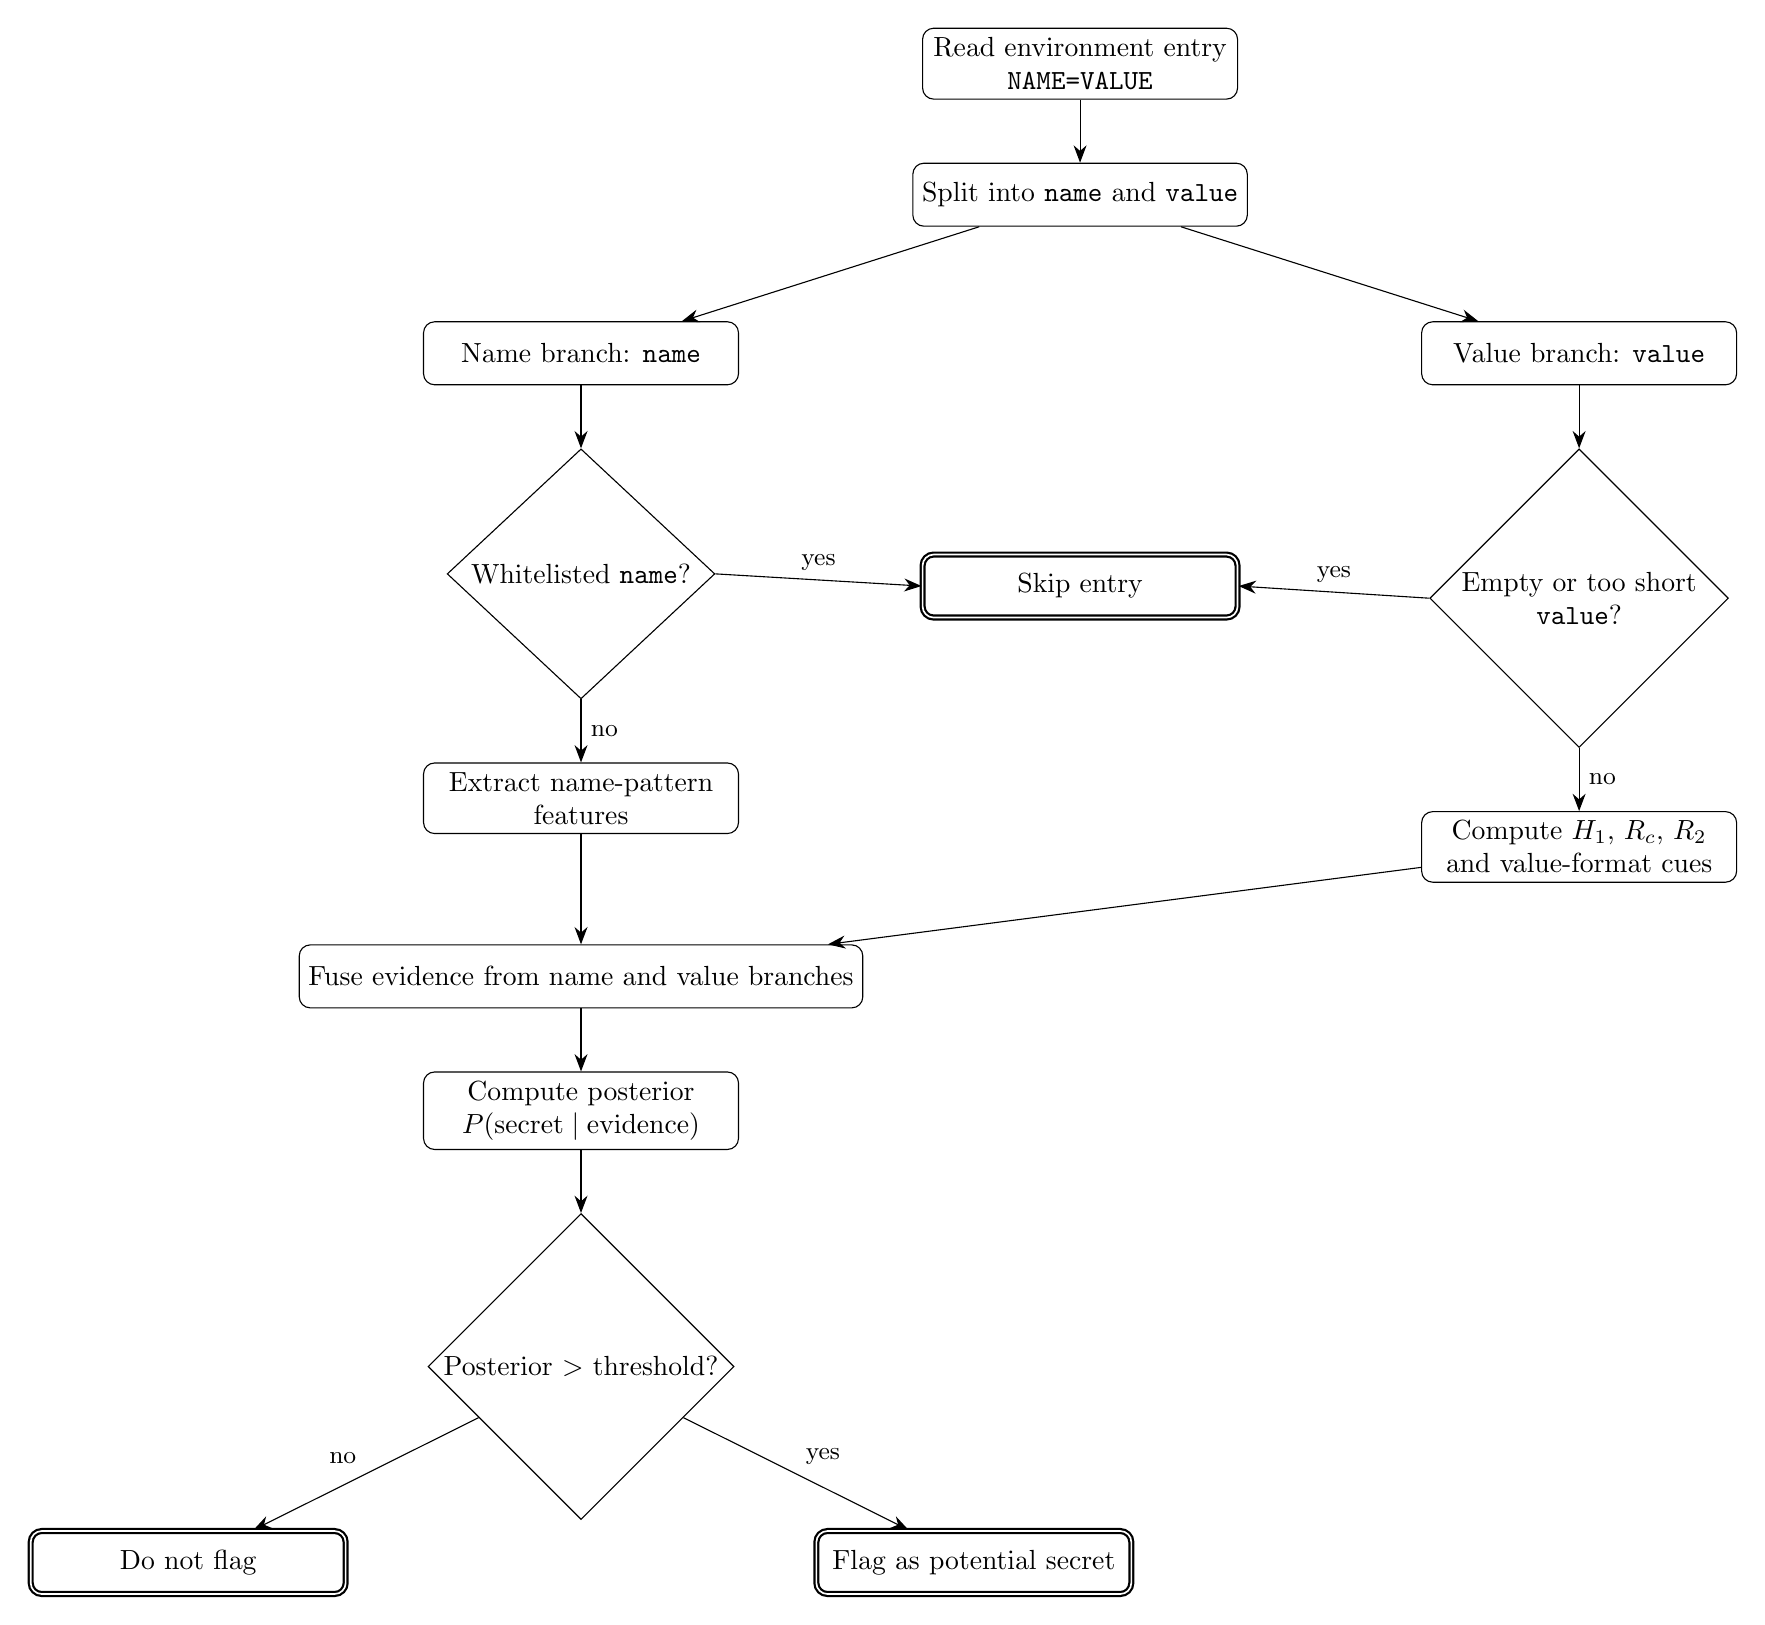
\begin{tikzpicture}[
  node distance=8mm and 10mm,
  box/.style={draw, rounded corners, align=center, minimum width=4.0cm, minimum height=8mm},
  terminal/.style={draw, rounded corners, align=center, minimum width=4.0cm, minimum height=8mm, thick, double},
  decision/.style={draw, diamond, align=center, inner sep=1pt, minimum width=3.4cm, minimum height=8mm},
  >={Stealth[length=2.2mm]}
]

\node[box] (start) {Read environment entry \\ \texttt{NAME=VALUE}};
\node[box, below=of start] (split) {Split into \texttt{name} and \texttt{value}};
\node[box, below left=12mm and 22mm of split] (namebranch) {Name branch: \texttt{name}};
\node[box, below right=12mm and 22mm of split] (valuebranch) {Value branch: \texttt{value}};
\node[decision, below=of namebranch] (whitelist) {Whitelisted \texttt{name}?};
\node[box, below=of whitelist] (namefeat) {Extract name-pattern \\ features};
\node[decision, below=of valuebranch] (lencheck) {Empty or too short \\ \texttt{value}?};
\node[box, below=of lencheck] (entropy) {Compute $H_1$, $R_c$, $R_2$ \\ and value-format cues};
\node[terminal] (skip) at ($(whitelist)!0.5!(lencheck)$) {Skip entry};
\node[box, below=14mm of namefeat] (fuse) {Fuse evidence from name and value branches};
\node[box, below=of fuse] (posterior) {Compute posterior \\ $P(\text{secret}\mid\text{evidence})$};
\node[decision, below=of posterior] (threshold) {Posterior $>$ threshold?};
\node[terminal, below left=11mm and 20mm of threshold] (notflag) {Do not flag};
\node[terminal, below right=11mm and 20mm of threshold] (flag) {Flag as potential secret};

\draw[->] (start) -- (split);
\draw[->] (split) -- (namebranch);
\draw[->] (split) -- (valuebranch);
\draw[->] (namebranch) -- (whitelist);
\draw[->] (whitelist) -- node[right, font=\small] {no} (namefeat);
\draw[->] (whitelist.east) -- node[above, font=\small] {yes} (skip.west);
\draw[->] (valuebranch) -- (lencheck);
\draw[->] (lencheck) -- node[right, font=\small] {no} (entropy);
\draw[->] (lencheck.west) -- node[above, font=\small] {yes} (skip.east);
\draw[->] (namefeat) -- (fuse);
\draw[->] (entropy) -- (fuse);
\draw[->] (fuse) -- (posterior);
\draw[->] (posterior) -- (threshold);
\draw[->] (threshold) -- node[above left, font=\small] {no} (notflag);
\draw[->] (threshold) -- node[above right, font=\small] {yes} (flag);

\end{tikzpicture}
}
\caption{Screening pipeline flow graph.}
\label{fig:screening-flow}
\end{figure}

\begin{table}[ht]
\centering
\begin{tabular}{|>{\raggedright\arraybackslash}p{4.1cm}|>{\raggedright\arraybackslash}p{2.3cm}|>{\raggedright\arraybackslash}p{6.3cm}|}
\hline
\textbf{Parameter} & \textbf{Default} & \textbf{Role} \\
\hline
Prior secret probability $P(\text{secret})$ & $0.10$ & Baseline posterior before evidence updates \\
\hline
Permutation count $B$ & $5$ or $10$ & Number of deterministic shuffles used for permutation baselines \\
\hline
Short-string cutoff & $12$ chars & Below cutoff, permutation-based entropy is skipped \\
\hline
Minimum value length for scoring & implementation-configured & Early prefilter to avoid unstable or non-informative scoring \\
\hline
Posterior flag threshold & deployment-configured & Decision boundary for ``flag as potential secret'' \\
\hline
\end{tabular}
\caption{Practical default parameters and their operational role.}
\label{tab:defaults}
\end{table}

\begin{algorithm}[ht]
\caption{Operational screening pseudocode}
\label{alg:screening}
\begin{algorithmic}[1]
\Require Environment entry \texttt{NAME=VALUE}, posterior threshold $\tau$
\Ensure One of \emph{Skip entry}, \emph{Do not flag}, \emph{Flag as potential secret}
\State Parse entry into \texttt{name} and \texttt{value}
\If{\texttt{name} is whitelisted}
  \State \Return \emph{Skip entry}
\EndIf
\If{\texttt{value} is empty or too short}
  \State \Return \emph{Skip entry}
\EndIf
\State Compute entropy features with short-string fallback:
\Statex \hspace{1.5em}$H_1 = -\sum_i p_i\log_2 p_i$, $R_c = \dfrac{H(X_i\mid X_{i-1})}{\operatorname{median}_{\pi} H(X_i^{\pi}\mid X_{i-1}^{\pi})}$, $R_2 = \dfrac{H_2(\text{original})}{\operatorname{median}_{\pi} H_2(\text{permuted})}$
\State Initialize posterior $P\gets P(\text{secret})=0.10$
\State Compute entropy likelihood pairs:
\Statex \hspace{1.5em}For each $r\in\{R_c,R_2\}$, let $d=|r-1|$ and set
\Statex \hspace{1.5em}$L_s^{r}=0.1+0.85\exp\!\left(-\tfrac12\left(\tfrac{r-1}{0.15}\right)^2\right)$,
\Statex \hspace{1.5em}$L_{\neg s}^{r}=\begin{cases}0.1,&d<0.3\\0.5+0.45\exp\!\left(-\tfrac12\left(\tfrac{d-0.3}{0.2}\right)^2\right),&d\ge 0.3\end{cases}$;
\Statex \hspace{1.5em}normalize Shannon entropy as $h=H_1/8$ and set
\Statex \hspace{1.5em}$L_s^{H_1}=\dfrac{1}{1+\exp(-10(h-0.6))}$, $L_{\neg s}^{H_1}=\dfrac{1}{1+\exp(-10(0.6-h))}$
\State For $e\in\{H_1,R_c,R_2\}$, update posterior with
\Statex \hspace{1.5em}$P \gets \dfrac{P\,L_s^{e}}{P\,L_s^{e} + (1-P)\,L_{\neg s}^{e}}$
\State Compute additional evidence: known prefix, name pattern, path-like indicator
\State Update posterior with additional evidence using
\Statex \hspace{1.5em}$P \gets \dfrac{P\,L_s}{P\,L_s + (1-P)\,L_{\neg s}}$
\If{posterior $> \tau$}
  \State \Return \emph{Flag as potential secret}
\Else
  \State \Return \emph{Do not flag}
\EndIf
\end{algorithmic}
\end{algorithm}

\section*{Failure Modes and Practical Checks}

Key failure modes and practical mitigations include:
\begin{itemize}
  \item \textbf{High-entropy non-secrets:} random identifiers that are not credentials may score high; mitigate with tighter name/prefix evidence.
  \item \textbf{Structured secrets:} secrets with strong formatting constraints may have lower entropy ratios; mitigate with prefix and name cues.
  \item \textbf{Path/value ambiguity:} uncommon path-like strings can be misclassified; mitigate by adjusting path heuristics for local environments.
  \item \textbf{Threshold drift:} operating point may shift across systems; mitigate by periodic threshold tuning on labeled samples.
\end{itemize}

\section*{Practical Characteristics}

\begin{itemize}
  \item \textbf{Interpretable:} each contribution is an explicit Bayesian update.
  \item \textbf{Deterministic:} permutation seeds are fixed by index, enabling reproducible scans.
  \item \textbf{Robust:} median over permutations reduces sensitivity to outlier shuffles.
  \item \textbf{Configurable:} threshold and minimum length can be tuned for precision/recall tradeoffs.
\end{itemize}

\section*{Summary}

This application note presents an implementation-oriented method for estimating secret probability in environment variables by combining permutation-aware entropy diagnostics with Bayesian evidence fusion over string statistics, naming cues, known prefixes, and path indicators. It further provides a practical hypothesis-testing interpretation, explicit assumptions and limitations, and reproducible screening defaults for operational pipelines.

\section*{References}

\textbf{[1]} W. Hoeffding, ``Probability Inequalities for Sums of Bounded Random Variables,'' \emph{Journal of the American Statistical Association}, vol. 58, no. 301, pp. 13--30, 1963.

\textbf{[2]} S. Boucheron, G. Lugosi, and P. Massart, \emph{Concentration Inequalities: A Nonasymptotic Theory of Independence}. Oxford University Press, 2013.

\textbf{[3]} K. Meli, M. McNiece, and B. Reaves, ``How Bad Can It Git? Characterizing Secret Leakage in Public GitHub Repositories,'' in \emph{Proceedings of the Network and Distributed System Security Symposium (NDSS)}, 2019.

\textbf{[4]} M. M. Rahman, C. Parnin, and L. Williams, ``Why Secret Detection Tools Are Not Enough: It's Not Just About False Positives,'' \emph{Empirical Software Engineering}, vol. 27, no. 3, 2022.

\textbf{[5]} GitHub Docs, ``About Secret Scanning,'' Accessed 2026. [Online]. Available: \texttt{https://docs.github.com/code-security/secret-scanning/about-secret-scanning}

\textbf{[6]} Yelp, ``detect-secrets,'' Accessed 2026. [Online]. Available: \texttt{https://github.com/Yelp/detect-secrets}

\textbf{[7]} Gitleaks Authors, ``gitleaks,'' Accessed 2026. [Online]. Available: \texttt{https://github.com/gitleaks/gitleaks}

\textbf{[8]} Z. Rice, ``Regex is (almost) all you need: How Gitleaks combines regex, entropy, and allowlists to find secrets,'' \emph{Looking at Computer}, Jan. 27, 2025.

\end{document}